\documentclass[a4paper,12pt,oneside,pdflatex,italian,final,twocolumn]{article}

\usepackage[utf8]{inputenc}
\usepackage{parallel}
\usepackage{siunitx}
\usepackage{booktabs}
\usepackage{fancyhdr}
\usepackage{subcaption}
\usepackage{listings}
\usepackage{hyperref}
\usepackage{pdfpages}
\usepackage{smartdiagram}
\usepackage{verbatim}

\usepackage[export]{adjustbox}
\usepackage[margin=0.5in]{geometry}
\addtolength{\topmargin}{0in}

\usepackage{libertine}
\renewcommand*\familydefault{\sfdefault}
\usepackage[T1]{fontenc}

\urlstyle{sf}
\hypersetup{
	colorlinks=true, %set true if you want colored links
	linktoc=all,     %set to all if you want both sections and subsections linked
	linkcolor=blue,  %choose some color if you want links to stand out
	urlcolor=blue,   %url color
}

\smartdiagramset{text width=2cm,module x sep= 3.4,back arrow disabled=true,}

\title{Smarthome Measurement Node Prototype}
\author{Achmadi ST MT}
\date{April 2023}

\begin{document}
	\pagestyle{fancy}

	\lhead{VibrasticLab}
	\chead{\today}
	\rhead{Specification Document v1.0}

	\onecolumn

	\begin{figure}

	\end{figure}\begin{minipage}{0.47\textwidth}
		\centering

	\end{minipage}
	\hfill
	\begin{minipage}{0.47\textwidth}
		\raggedleft
		\Huge \textbf{Smarthome Measurement Node}
	\end{minipage}

	\begin{figure}
		\begin{minipage}{0.47\textwidth}

			\section{Overview}
			\begin{itemize}
				\item Battery AAA Operated
				\item Low-Power WiFi Cient
				\item Re-Programmable Firmware
				\item Analog, I2S, and I2C interfaces
				\item Indicator LEDs Array
			\end{itemize}


		\end{minipage}
		\hfill
		\begin{minipage}{0.47\textwidth}
			\centering
			\includegraphics[width=0.7\textwidth,right]{images/view_ortho.png}

	\end{minipage}
	\end{figure}

	\raggedright
	\section{Main Unit Part}

	\centering
	\begin{figure}[!ht]
		\centering
		\includegraphics[width=\textwidth,]{images/node_part.png}
		\caption{Prototype Unit Parts}
	\end{figure}

	\raggedright
	\section{Data Exchange Flow}

	\smartdiagram[flow diagram:horizontal]{Multi Sensor Node,
		MQTT or HTTP Server, Data Bank Server, Data Fetch API, Python or Matlab Analysis}\\

	\vspace{10pt}

	\textbf{NOTES:} Its recommended to use Local Server infrastructure, preferably in accessable server room during development phase.

	\raggedright
	\section{PCB Design}

	\newpage
	\includepdf[pages=-,angle=-90]{pdf/nodemcu_based.pdf}

	\newpage
	\includepdf[pages=-,angle=-90]{pdf/bom.pdf}

	\raggedright
	\section{Project Repository}

	Current project repository: \href{https://github.com/VibrasticLab/smarthome_proto}{Github VibrasticLab}

	\raggedright
	\section{Development Constraints/Obstacles}

	Some development constraints/obstacles:

	\begin{itemize}
		\item Time span, including: PCB building time, firmware implementation, testing and calibration, server building.

		\item Calibration process, including: standards, controlled test environment, and already available measurement tools.

		\item Personel requirement, including: programmers (either embedded or backend server), project managers/administrator, purchasing staff, etc.

		\item Components handling, for example:

		\begin{itemize}
			\item MG-811 CO2 sensor requires heating to operate, thus consume high power from battery.

			\item Light Intensity might influenced by placement angle.
		\end{itemize}

	\end{itemize}

	\raggedright
	\section{Cost Estimation}

	\subsection{Unit Cost}

	\begin{tabular}{|l|l|l|}
		\toprule
		Item & Price-Qty & URL \\
		\midrule
		NodeMCU ESP32 & Rp. 66.800 & \href{https://www.tokopedia.com/temins/esp32-esp-32-arduino-wifi-bluetooth-iot-development-board-micro-usb}{Tokped} \\
		HTU21D & Rp. 35.000 & \href{https://www.tokopedia.com/akhishop/htu21d-temperature-and-humidity-sensor-module}{Tokped} \\
		BH1750 & Rp. 20.000 & \href{https://www.tokopedia.com/akhishop/gy-302-light-intensity-bh1750-module-sensor-intensitas-cahaya}{Tokped} \\
		\midrule
		Total & Rp. 674.100  & - \\
		\bottomrule
	\end{tabular}

\end{document}